\documentclass[journal]{IEEEtran}

\usepackage{amsmath,amssymb}
\usepackage{graphicx}
\usepackage{booktabs}
\usepackage{multirow}
\usepackage{cite}
\usepackage{url}
\usepackage[hidelinks]{hyperref}
\usepackage{xcolor}
\usepackage{tikz}
\usetikzlibrary{arrows.meta,positioning,fit}

\newcommand{\method}{DisasterSociety}
\newcommand{\R}{\mathbb{R}}

\tikzset{
  block/.style={
    draw,
    rounded corners=2pt,
    align=center,
    minimum height=7mm,
    text width=25mm,
    font=\footnotesize,
    fill=blue!5
  },
  module/.style={
    draw,
    rounded corners=2pt,
    align=center,
    minimum height=7mm,
    text width=28mm,
    font=\footnotesize,
    fill=green!7
  },
  data/.style={
    draw,
    rounded corners=2pt,
    align=center,
    minimum height=7mm,
    text width=23mm,
    font=\footnotesize,
    fill=orange!10
  },
  flow/.style={-{Latex[length=2mm]}, thick},
  dashedflow/.style={-{Latex[length=2mm]}, thick, dashed}
}

\begin{document}

\title{DisasterSociety: Population-Calibrated Persistent Agents for
Cross-Hazard Protective-Action Simulation}

\author{Anonymous Author(s)%
\thanks{Author names, affiliations, funding information, and the corresponding
author will be added after the target journal and review policy are fixed.}}

\markboth{IEEE Transactions Journal Draft, July 2026}%
{Anonymous Author(s): DisasterSociety}

\maketitle

\begin{abstract}
Post-disaster surveys usually retain whether and when households take
protective action, but observe the preceding sequence of warnings, appraisals,
preparation, coordination, and execution only partially and heterogeneously.
Statistical models can estimate outcome and time distributions without
generating this process; large language model (LLM) agents can generate
detailed trajectories, but plausible narratives alone do not guarantee
population calibration, temporal legality, or bounded information access. We
formulate disaster
protective-action simulation as population-calibrated causal event-history
generation and present \method, a generative multi-agent framework that
separates calibration from process generation. Hazard and dataset adapters
map event-specific evidence and survey fields into shared contracts. A
persistent household agent updates cognitive and coordination states
structured by the Protective Action Decision Model using only time-bounded,
provenance-aware evidence, while a statistical event-history layer controls
finite-window outcome and departure risk. A deterministic executor enforces
legal state transitions and
records complete evidence-to-action traces. The resulting research object is
not respondent-level label prediction or narrative replay of a known disaster,
but a joint distribution of auditable household histories. We define a
multi-level evaluation protocol using Hurricane Irma and Carr Fire event packs
that separately tests population and subgroup distributions, departure timing,
causal and legal validity, retrospective Irma-to-Carr cross-hazard
confirmation under frozen methods, and the functional effects of persistence,
memory, feedback, and planning. This formulation makes cognitive modules
falsifiable mechanisms and allows LLM-generated social processes to be
assessed without treating classification accuracy as their primary measure.
\end{abstract}

\begin{IEEEkeywords}
Generative agents, multi-agent simulation, disaster evacuation, protective
action, cognitive modeling, event history, calibration, cross-hazard
validation.
\end{IEEEkeywords}

\section{Introduction}
\IEEEPARstart{H}{ousehold} protective action during a wildfire or hurricane
develops over time. A household receives partial information, judges the
source, assesses personal threat, checks transport and dependent-care
constraints, prepares, and then departs or remains in place. A final
evacuation label omits this history. Departure time alone also omits why a
household became ready at that point.

Statistical choice and event-history models provide calibrated estimates of
evacuation probability and departure time. They remain the appropriate
reference when the task is supervised prediction. Their compact state,
however, does not produce a causal sequence of observations, appraisals,
preparation actions, execution results, and later revisions. Rule-based
agent-based models (ABMs) add temporal state and interaction
\cite{bonabeau2002agent,macal2010tutorial}, but their behavioral transitions
must be explicitly specified by the modeler.

Large language models (LLMs) offer a different kind of process model.
LLM-based generative agents can retain memories, synthesize reflections, and
plan behavior across multi-step interactions \cite{park2023generative}.
Platforms such as GenSim and AgentSociety extend this approach to large
populations and reusable social environments
\cite{tang2024gensim,piao2025agentsociety}. Disaster applications have also
begun to combine behavioral theory with LLM reasoning; FLARE, for example,
predicts wildfire evacuation decisions from post-event survey records
\cite{chen2025flare}. Yet generative detail does not resolve empirical
validity by itself. High-stakes crowd simulation therefore requires explicit
evaluation of whether language-agent behavior aligns with observed human
behavior \cite{wang2025alignment}; process fidelity depends on variability and
adaptation rather than a preferred action alone
\cite{feng2025fidelity}; and an agent can appear more capable when it is given
an unrealistically omniscient view of the interaction
\cite{zhou2024fantasy}. A fluent trajectory is therefore not sufficient
evidence that a simulated population or decision process is valid.

In this work, we study \emph{population-calibrated causal event-history
generation} for disaster protective action. Given a time-stamped exogenous
event stream and pre-decision household attributes, the task is to generate a
joint population of histories, realized protective-action outcomes, and event
times. A valid generator must satisfy three requirements. First, its aggregate
and conditional outcome and timing distributions must remain anchored to
observed data. Second, each household history must respect information
availability and legal action ordering. Third, every simulated outcome must be
traceable to delivered evidence, evolving appraisal, preparation or
coordination, and execution. This task is neither respondent-level label
prediction nor narrative reconstruction of a known disaster. Hurricane Irma
and the Carr Fire serve as validation event packs for a reusable framework,
not as the scope of the framework itself.

Three challenges follow from this formulation. The first is to connect
population constraints to generated histories without preassigning a hidden
binary outcome or exposing fitted probabilities to the agent. The second is
to preserve causal state across time: environmental truth, household
observation, and household belief must remain distinct, and no proposed action
may bypass its prerequisites. The third is to separate reusable behavioral
contracts from event-specific base rates, timing, and evidence semantics while
testing each cognitive component against the function it is intended to
provide. In particular, memory, execution feedback, and planning cannot be
treated as contributions merely because they are present in the architecture.

\method{} assigns these responsibilities to separate system components.
Dataset and hazard adapters map heterogeneous surveys and event records to a
shared household, evidence, and action schema. A training-fitted statistical
layer supplies continuous household propensity and discrete-time event risk
without revealing either quantity to the agent. A persistent agent constrained
by the Protective Action Decision Model (PADM) updates appraisal, preparation,
coordination, and readiness using only evidence delivered by the current
simulation time. A deterministic executor
then enforces action legality, realizes permitted transitions, and writes the
result back to the next agent state. Outcomes and event times are read from
the executed history rather than inserted into the prompt or forced at the end
of the simulation. Complete logs expose disagreements among calibrated risk,
agent readiness, and realized action for later diagnosis.

We make three contributions.
\begin{enumerate}
    \item We formulate disaster protective-action simulation as
    population-calibrated causal event-history generation, with population
    distribution, event timing, and process validity defined as separate
    empirical objects (Section~\ref{sec:problem}).
    \item We develop a calibration--generation architecture that combines
    event-pack adapters, bounded perception, persistent PADM appraisal,
    statistical event risk, a legal executor, and complete causal logs
    (Section~\ref{sec:framework}). Optional cognitive and social components
    are exposed as falsifiable mechanisms rather than assumed improvements.
    \item We define a multi-level evaluation protocol using wildfire and
    hurricane event packs, statistical and agent-based baselines, paired
    mechanism ablations, and separate distributional, temporal, process, and
    cross-hazard criteria (Section~\ref{sec:experiments}). Individual
    classification is retained only as a secondary diagnostic.
\end{enumerate}

\section{Related Work}
Our problem lies at the intersection of protective-action theory, sequential
agent simulation, and empirical model validation. We organize prior work by
the empirical object it explains: a final choice, a decision trajectory, or a
population distribution of trajectories.

\subsection{Protective Action, Evacuation, and Event Histories}
The Protective Action Decision Model (PADM) separates environmental and
social cues, predecision processes, threat, protective-action, and stakeholder
perceptions, and situational facilitators and impediments
\cite{lindell2012padm}. This decomposition is important because a household
can receive evidence without believing it, believe a threat without having a
feasible action, or become ready without departing immediately. Statistical
choice models summarize the resulting
stay-or-go outcome, whereas survival and event-history models represent the
timing of an event conditional on remaining at risk
\cite{cox1972regression}. Wildfire studies have consequently examined both
evacuation choice and departure timing \cite{toledo2018analysis}. Reviews of
wildfire evacuation simulation further identify heterogeneous response,
behavioral-data scarcity, and the coupling of behavioral and traffic models
as persistent challenges \cite{beyki2023evacuation}.

These traditions provide the behavioral variables and population-level
targets needed for validation; they are not merely baselines to be displaced
by an LLM. Their usual empirical outputs, however, are choices, hazards, or
aggregate traffic patterns rather than auditable evidence-to-appraisal-to-
action histories. \method{} therefore retains statistical outcome and timing
models as constraints while using a generative policy only for the
intermediate, temporally ordered process.

\subsection{Persistent Generative Agents and Social Simulation}
Generative Agents introduced a memory--reflection--planning architecture for
long-horizon social behavior \cite{park2023generative}. Subsequent platforms
have emphasized reusable environments and simulation infrastructure. GenSim
supports customized scenarios, large populations, and long-run error
correction \cite{tang2024gensim}; AgentSociety combines LLM-driven agents,
realistic urban environments, and computational social experiments
\cite{piao2025agentsociety}. The broader literature now spans cyber, physical,
social, and hybrid systems, while continuing to identify perception, human
alignment, action generation, and evaluation as open problems
\cite{gao2023llmabm}.

This line of work establishes that persistent state and environmental
interaction can produce coherent multi-step behavior. It does not imply that
memory, feedback, or planning automatically improves empirical validity.
For disaster simulation, each component must instead be connected to an
observable function---for example, recall continuity, response to execution
failure, or consistency of plan revision---and tested at the trajectory level.
Our focus is consequently not a more general agent platform, but a controlled
way to turn persistent agents into population-calibrated event-history
generators.

\subsection{Behavioral Alignment and Multi-Level Validation}
Recent work makes the behavior-realism problem explicit. Persona-Environment
Behavioral Alignment formulates high-stakes crowd simulation as distribution
matching and iteratively refines personas against expert behavioral
benchmarks \cite{wang2025alignment}. Process-oriented evaluation further shows
that matching a preferred action is insufficient when agents fail to
reproduce human variability and adaptation across rounds
\cite{feng2025fidelity}. Information access is another validity boundary:
LLM agents evaluated in omniscient settings can appear more successful than
the same agents operating under realistic information asymmetry
\cite{zhou2024fantasy}.

These concerns parallel established ABM validation practice. Pattern-oriented
calibration compares a model against multiple weak patterns; in a
protective-behavior case study, fitting both the magnitude and timing of
adoption exposed structural flaws hidden by a single error criterion
\cite{badham2017calibrating}. VALFRAM likewise validates generated schedules
along temporal, spatial, and structural dimensions rather than reducing an
activity history to one endpoint \cite{drchal2016valfram}. Taken together,
this work argues against using either individual accuracy or narrative
plausibility as a sufficient statistic. \method{} follows the multi-level
principle but couples three objects that are commonly evaluated separately:
the population outcome distribution, the departure-time distribution, and
the legality and causal coherence of each generated history.

\subsection{LLMs for Disaster and Emergency Behavior}
Disaster-specific LLM research is moving from unconstrained role play toward
behavioral structure. FLARE integrates behavioral theory, chain-of-thought
reasoning, and memory-based reinforcement learning to predict individual
wildfire evacuation decisions from post-event survey records
\cite{chen2025flare}. Hierarchical Generative Agents model evacuation as
sequential high-level goal setting, route reasoning, and low-level navigation,
with calibration to empirical evacuation data
\cite{mendoza2026hierarchical}. PAVE addresses a complementary emergency
problem: it structures how agents perceive, assess, delimit, and recover from
legitimate rule violations, and evaluates properties such as authority
deference and bounded scope \cite{yehia2026pave}.

The closest work thus offers, respectively, theory-informed outcome
prediction, cognitively structured evacuation and navigation, or
property-based emergency reasoning. \method{} changes the primary empirical
object to a joint population of household event histories. A separate
calibration layer constrains finite-window outcomes and timing; the persistent
agent generates only causally available observation--appraisal--action
transitions; and the executor makes every transition auditable. This
calibration--generation separation is the methodological distinction on which
the remainder of the paper builds.

\section{Problem Formulation}
\label{sec:problem}
Let the simulation window contain ticks $t=0,\ldots,T-1$ and households
$\mathcal{V}=\{1,\ldots,N\}$. The exogenous event stream is
\begin{equation}
\mathcal{E}_{0:T}=\{e_k\}_{k=1}^{K},
\end{equation}
where each event contains a publication time, type, geographic scope, source,
provenance, and uncertainty. Household $i$ has pre-decision attributes $X_i$,
including household composition, mobility constraints, vehicle access,
previous experience, information access, and coarse location.

The simulator generates
\begin{equation}
\{\mathcal{H}_i,Y_i,\tau_i\}_{i=1}^{N},
\end{equation}
where $\mathcal{H}_i$ is an evidence-to-action history, $Y_i$ is the
finite-window protective-action outcome, and $\tau_i$ is the simulated
departure time if departure occurs. An explicit stayer is a complete
finite-window non-event. Only an incomplete survey history is right-censored.

Environmental truth, household observation, and household belief remain
distinct:
\begin{equation}
W_t \neq O_{i,t} \neq B_{i,t}.
\label{eq:truth-observation-belief}
\end{equation}
An event can enter $O_{i,t}$ only if it has been published by $t$, is relevant
to the household, and passes the configured delivery rule. The policy cannot
observe the survey outcome, observed departure time, fitted propensity, random
draw, or future event.

The empirical objective has three parts:
\begin{align}
\mathcal{L}_{outcome} &=
  d\!\left(\widehat{P}(Y),P_{survey}(Y)\right),\\
\mathcal{L}_{time} &=
  d\!\left(\widehat{P}(\tau),P_{survey}(\tau)\right),\\
\mathcal{L}_{process} &=
  \phi(\{\mathcal{H}_i\}),
\end{align}
where $d$ denotes distributional or calibration error and $\phi$ contains
legality, temporal-causality, and mechanism diagnostics. No single
classification metric is used as evidence for all three parts.

\section{The \method{} Framework}
\label{sec:framework}
\subsection{System Boundary and Adapters}
Fig.~\ref{fig:overview} shows the framework boundary. A dataset adapter maps
heterogeneous survey variables to a common household and outcome schema. A
hazard adapter maps official orders and public hazard records to typed,
timestamped evidence. The universal simulator reads only the common schema.
Outcome fields remain in the evaluation store and cannot enter the agent
observation.

\begin{figure*}[!t]
\centering
\resizebox{\textwidth}{!}{%
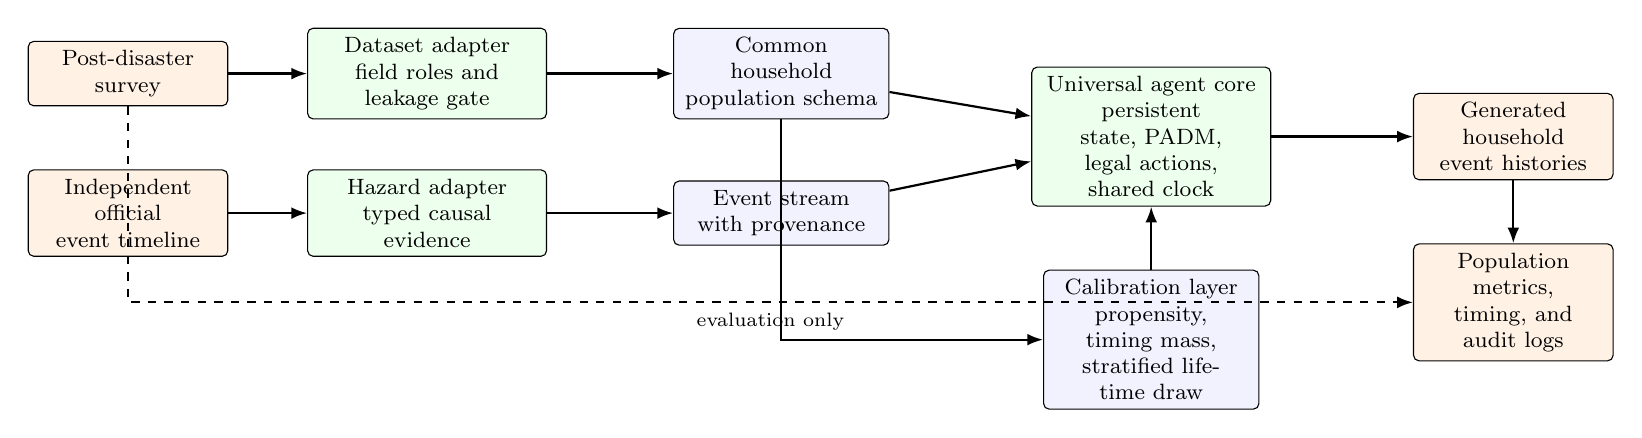
\begin{tikzpicture}[node distance=8mm and 10mm]
  \node[data] (survey) {Post-disaster\\survey};
  \node[data, below=of survey] (official) {Independent official\\event timeline};
  \node[module, right=of survey] (dataset) {Dataset adapter\\field roles and leakage gate};
  \node[module, right=of official] (hazard) {Hazard adapter\\typed causal evidence};
  \node[block, right=16mm of dataset] (population) {Common household\\population schema};
  \node[block, right=16mm of hazard] (events) {Event stream\\with provenance};
  \node[module, right=18mm of population, yshift=-8mm] (core) {Universal agent core\\persistent state, PADM,\\legal actions, shared clock};
  \node[block, below=8mm of core] (calibration) {Calibration layer\\propensity, timing mass,\\stratified lifetime draw};
  \node[data, right=18mm of core] (history) {Generated household\\event histories};
  \node[data, below=of history] (audit) {Population metrics,\\timing, and audit logs};

  \draw[flow] (survey) -- (dataset);
  \draw[flow] (official) -- (hazard);
  \draw[flow] (dataset) -- (population);
  \draw[flow] (hazard) -- (events);
  \draw[flow] (population) -- (core);
  \draw[flow] (events) -- (core);
  \draw[flow] (population) |- (calibration);
  \draw[flow] (calibration) -- (core);
  \draw[flow] (core) -- (history);
  \draw[flow] (history) -- (audit);
  \draw[dashedflow] (survey) |- node[pos=0.75, below, font=\scriptsize]
    {evaluation only} (audit);
\end{tikzpicture}
}
\caption{System boundary. Survey outcomes are separated from agent inputs.
Hazard and dataset adapters feed a shared agent core; the calibration layer
controls outcome and timing mass without exposing hidden targets to agents.}
\label{fig:overview}
\end{figure*}

\subsection{Training-Fitted Household Propensity}
A regularized contextual logistic model is fitted on the source training
partition:
\begin{equation}
p_i=P(Y_i=1\mid X_i)
    =\sigma(\beta_0+\beta^\top X_i).
\label{eq:propensity}
\end{equation}
The features cover household composition, home-area context, mobility and
transport, information access, age, and decision role. Missing values are
imputed within the training pipeline. The resulting $p_i$ is continuous. It
is never converted into a fixed binary eligibility class and is hidden from
the agent.

For target-training-only robustness analysis, we preserve the source-trained
slopes and ranking and fit one intercept on the target training split:
\begin{equation}
p_i^{(a)}=\sigma\!\left(\operatorname{logit}(p_i)+a\right).
\label{eq:intercept-adapter}
\end{equation}
The Carr test split is excluded when estimating $a$. This adapter measures
whether a small hazard-specific base-rate parameter can repair cross-event
calibration. It is not reported as zero-shot transfer.

\subsection{Training-Fitted Timing Mass}
Let $w_t\geq0$ be the fraction of observed training departures in tick $t$,
with Jeffreys smoothing:
\begin{equation}
w_t=\frac{n_t+1/2}{\sum_{s=0}^{T-1}n_s+T/2},
\qquad \sum_{t=0}^{T-1}w_t=1.
\label{eq:timing-weight}
\end{equation}
The Irma-trained weights define the frozen cross-hazard timing condition. A
Carr-training-only timing adapter replaces $\{w_t\}$ while keeping the agent
core and household propensity slopes fixed. We also test Gaussian smoothing
over timing bins. Five-fold likelihood selection on Carr training data chooses
zero smoothing, so the smoothed variant is rejected before test
interpretation.

\subsection{Legal-Risk-Set Deferred Mass}
The main controller consumes timing mass only when the household is in
\texttt{PREPARING} or \texttt{COORDINATING}. Let $L_{i,t}\in\{0,1\}$ indicate
membership in this legal pre-departure risk set. Let $d_{i,t}^{-}$ be timing
mass deferred before tick $t$ and $c_{i,t}^{-}$ be mass already consumed. The
effective mass is
\begin{equation}
q_{i,t}=
\begin{cases}
\min(1-c_{i,t}^{-},w_t+d_{i,t}^{-}),&L_{i,t}=1,\\
0,&L_{i,t}=0.
\end{cases}
\label{eq:effective-mass}
\end{equation}
The update is
\begin{align}
d_{i,t}^{+}&=
\begin{cases}
0,&L_{i,t}=1,\\
\min(1-c_{i,t}^{-},d_{i,t}^{-}+w_t),&L_{i,t}=0,
\end{cases}\\
c_{i,t}^{+}&=\min(1,c_{i,t}^{-}+q_{i,t}).
\label{eq:mass-update}
\end{align}
The corresponding conditional hazard, retained in the audit log, is
\begin{equation}
h_{i,t}=\frac{p_iq_{i,t}}{1-p_ic_{i,t}^{-}}.
\label{eq:conditional-hazard}
\end{equation}
This construction does not create an invisible pending departure. A household
that is not ready accumulates timing mass; the mass becomes available at the
next legal tick. A household that never reaches the risk set remains a process
non-event, exposing disagreement between the calibrated outcome head and the
generated preparation process.

\subsection{Variance-Controlled Lifetime Realization}
Each household receives one lifetime uniform draw. For $K=5$ registered seeds,
a stable household hash supplies an offset $o_i\in\{0,\ldots,K-1\}$ and jitter
$j_i\in[0,1)$. Run $s$ uses
\begin{equation}
u_{i,s}=\frac{(s+o_i)\bmod K+j_i}{K}.
\label{eq:lhs-draw}
\end{equation}
The five runs therefore place each household once in every uniform stratum,
as in Latin-hypercube sampling \cite{mckay1979lhs}. Departure occurs at the
first legal tick satisfying
\begin{equation}
u_{i,s}<p_i c_{i,t}^{+}.
\label{eq:departure-trigger}
\end{equation}
This reduces five-seed Monte Carlo noise while preserving the marginal
lifetime probability $p_i$. The same hash and registered seeds are used in
all paired comparisons.

\subsection{Persistent Agent State and PADM Appraisal}
At tick $t$, agent $i$ maintains
\begin{equation}
S_{i,t}=(X_i,D_{i,t},B_{i,t},M_{i,t},P_{i,t}),
\end{equation}
where $D_{i,t}$ is objective dynamic state, $B_{i,t}$ is structured PADM
appraisal, $M_{i,t}$ is optional structured memory, and $P_{i,t}$ is an
optional short plan. The main evaluation profile persists the legal stage and
PADM state. A separate mechanism ablation activates execution feedback,
memory, and plan revision.

The observation includes only evidence delivered by the current tick. Each
item retains time, source, credibility, geographic relevance, and provenance.
The policy updates threat appraisal, protective-action feasibility and cost,
source trust, contradictions, and a readiness value in
\{\texttt{not\_ready}, \texttt{considering}, \texttt{ready}\}. It returns one
JSON object containing a legal action, intended stage, readiness, rationale,
cited evidence identifiers, a plan of at most three steps, and optional
messages. Citations not present in the current observation are removed.

\subsection{Action State Machine and Execution}
The action state machine includes
\begin{equation}
\begin{aligned}
\texttt{UNAWARE}&\rightarrow\texttt{MONITORING}\\
&\rightarrow\texttt{PREPARING}
\leftrightarrow\texttt{COORDINATING}\\
&\rightarrow\texttt{DEPARTING}
\rightarrow\texttt{EVACUATED},
\end{aligned}
\end{equation}
with legal finite-window branches to \texttt{STAYING}. A policy may declare
readiness, but it cannot force departure while the controller is active. The
executor checks action-stage compatibility, commits the legal transition, and
records acceptance, rejection, objective updates, and completion.

\subsection{Synchronous Concurrent Kernel}
All households share one simulation clock. At each tick the engine:
\begin{enumerate}
    \item replays exogenous events and delivers due messages;
    \item freezes a read-only world snapshot;
    \item constructs bounded observations;
    \item runs household decisions concurrently;
    \item waits at a barrier before any decision can affect another;
    \item applies the departure controller and validates actions;
    \item commits transitions and queues later messages;
    \item writes the causal trajectory and validity audit.
\end{enumerate}
The experiments use up to 32 concurrent model calls. Concurrency changes wall
time, not simulated time. A message created at tick $t$ cannot affect another
agent inside that tick.

\begin{figure*}[!t]
\centering
\resizebox{\textwidth}{!}{%
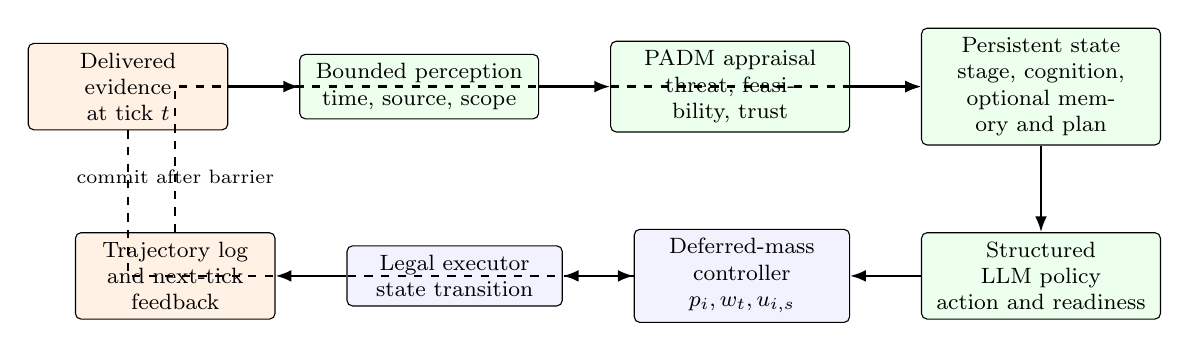
\begin{tikzpicture}[node distance=8mm and 9mm]
  \node[data] (event) {Delivered evidence\\at tick $t$};
  \node[module, right=of event] (perception) {Bounded perception\\time, source, scope};
  \node[module, right=of perception] (padm) {PADM appraisal\\threat, feasibility, trust};
  \node[module, right=of padm] (state) {Persistent state\\stage, cognition,\\optional memory and plan};
  \node[module, below=11mm of state] (policy) {Structured LLM policy\\action and readiness};
  \node[block, left=of policy] (controller) {Deferred-mass controller\\$p_i,w_t,u_{i,s}$};
  \node[block, left=of controller] (executor) {Legal executor\\state transition};
  \node[data, left=of executor] (log) {Trajectory log\\and next-tick feedback};

  \draw[flow] (event) -- (perception);
  \draw[flow] (perception) -- (padm);
  \draw[flow] (padm) -- (state);
  \draw[flow] (state) -- (policy);
  \draw[flow] (policy) -- (controller);
  \draw[flow] (controller) -- (executor);
  \draw[flow] (executor) -- (log);
  \draw[dashedflow] (log) |- node[pos=0.25, below, font=\scriptsize]
    {commit after barrier} (state);
  \draw[dashedflow] (event) |- (controller);
\end{tikzpicture}
}
\caption{Household decision and execution loop. The agent controls cognition,
preparation, and readiness. The calibration layer controls event realization,
and the executor enforces legal transitions.}
\label{fig:agent}
\end{figure*}

\subsection{Audit and Validity Gates}
Every transition stores the observation, cognition before and after, retrieved
memories, proposed action, controlled action, execution result, and departure
control record. Every model call stores the prompt hash, seed, status, token
counts, latency, and cache status. Outputs are validated against a typed
schema. A malformed response receives one repair attempt; a failed request
falls back to a rule policy and is recorded. A run is invalid if fallback
exceeds 1\%, an output is missing, a future event enters an observation, or an
illegal transition exceeds the registered tolerance.

\section{Experimental Design}
\label{sec:experiments}
\subsection{Data and Evaluation Cohorts}
Table~\ref{tab:data} summarizes the two event packs. The Irma survey contains
1,263 valid responses and 921 completed questionnaires. Official evacuation
orders come from the Hurricane Evacuation Order Database. The formal
within-event test uses the Brevard County public-signal cohort associated with
HEvOD event 21: 87 households, including 42 evacuees and 45 stayers.

The Carr survey contains 330 valid stay-or-go responses among completed
records, with 293 evacuees and 37 stayers, and 292 complete departure times.
The retrospective Carr test contains 68 households, including 60 evacuees and
eight stayers. Carr-train adapter experiments use 197 training households;
the test split remains evaluation-only. Independent CAL FIRE records provide
the public event timeline.

\begin{table}[!t]
\caption{Event Packs and Formal Evaluation Cohorts}
\label{tab:data}
\centering
\small
\begin{tabular}{lcc}
\toprule
 & Irma 2017 & Carr Fire 2018\\
\midrule
Valid raw responses & 1,263 & 647\\
Completed questionnaires & 921 & 335\\
Valid stay/go outcome & 917 & 330\\
Complete departure time & 539 & 292\\
Formal test households & 87 & 68\\
Formal test evacuated & 42 & 60\\
Formal test stayed & 45 & 8\\
External event source & HEvOD & CAL FIRE\\
\bottomrule
\end{tabular}
\end{table}

The surveys are convenience samples. We report survey-conditioned
reconstruction, not county or state population estimates. Exact respondent
locations, observed social ties, respondent GPS trajectories, and link-level
traffic measurements are unavailable.

\subsection{Splits, Leakage Control, and Freezing}
Each event pack uses a household-stratified split with seed 42. All records
derived from one respondent remain in the same partition. Survey outcomes,
departure times, and post-decision fields are tagged as targets or diagnostics
and cannot enter the policy prompt. The Irma training partition fits the
contextual propensity and frozen timing weights. Development experiments
select the calibrated deferred-mass controller and state-only profile before
the Irma test summary is generated.

Carr is not described as a pristine external validation because the project
had inspected it before the final protocol. We call it retrospective
cross-hazard confirmation after method freezing. The frozen condition uses
Irma propensity and timing components without Carr labels. Separate
target-training-only robustness conditions fit an intercept and timing weights
on Carr train and never use Carr test labels.

\subsection{Baselines and Ablations}
The within-Irma comparison includes:
\begin{enumerate}
    \item a regularized logistic outcome model;
    \item a contextual propensity model using harmonized household features;
    \item a non-LLM PADM rule ABM;
    \item a one-shot stateless LLM;
    \item the calibrated persistent process.
\end{enumerate}
All LLM experiments use \texttt{deepseek-v4-flash} through an
OpenAI-compatible interface, temperature 0.2, structured JSON output, and
registered seeds 41--45. We report model-call counts and output validity for
computational reproducibility.

The mechanism ablation uses a frozen 30-household Irma subset and four
cumulative profiles:
stateless, state-only, state plus execution feedback, and full-persistent with
structured memory and plan revision. Each profile uses five paired seeds. This
design tests whether named modules change empirical outcomes; architectural
availability alone is not counted as evidence.

\subsection{Metrics and Uncertainty}
Outcome metrics are Macro-F1, balanced accuracy, Brier score, expected
calibration error (ECE), and absolute population-share error. We report
individual discrimination as a diagnostic because the primary object is the
population event-history distribution. Five-seed ensemble probabilities equal
the household's realized action frequency across seeds.

Departure-time metrics are Wasserstein-1 distance in hours, integrated absolute
difference between empirical cumulative distribution functions (CDF IAE), and
absolute mean-time error. Process metrics include illegal-transition rate,
future-evidence count, fallback rate, PADM evidence response, source-appraisal
coverage, readiness-to-execution diagnostics, repeated actions, feedback
response, and plan revision.

Household-level effects use 10,000 paired bootstrap samples. Timing-adapter
effects use paired seed statistics. We report point effects and 95\% percentile
intervals. An interval crossing zero is treated as inconclusive, regardless of
the direction of the point estimate.

\subsection{Evaluation Structure}
\begin{table}[!t]
\caption{Empirical Evaluation Components}
\label{tab:matrix}
\centering
\small
\begin{tabular}{p{0.29\columnwidth}p{0.61\columnwidth}}
\toprule
Component & Empirical purpose\\
\midrule
Data validity & Schema, provenance, split, and leakage checks\\
Irma reconstruction & Within-event outcome and timing evaluation\\
Mechanism ablation & Persistent state, feedback, memory, and planning\\
Frozen transfer & Retrospective Irma-to-Carr confirmation\\
Target-train robustness & Carr intercept, timing, and resolution adapters\\
Process validity & Sequence legality and causal-information checks\\
\bottomrule
\end{tabular}
\end{table}

\section{Results}
\subsection{Irma Within-Event Reconstruction}
Table~\ref{tab:irma-main} reports the 87-household Irma test. The calibrated
persistent ensemble
has the highest Macro-F1 (0.551), balanced accuracy (0.553), and lowest
population-share error (0.018). The contextual propensity has a lower Brier
score (0.261 versus 0.269), while the persistent ensemble has lower ECE
(0.124 versus 0.154).

\begin{table*}[!t]
\caption{Irma Test Results on the Frozen 87-Household Cohort}
\label{tab:irma-main}
\centering
\small
\begin{tabular}{lcccccc}
\toprule
Method & Runs & Macro-F1 & Bal. Acc. & Brier & ECE & Share error\\
\midrule
Logistic outcome model & 1 & 0.490 & 0.539 & \textbf{0.248} & -- & 0.096\\
Contextual propensity & 1 & 0.494 & 0.496 & 0.261 & 0.154 & 0.045\\
PADM rule ABM & 5 & 0.326 & 0.500 & 0.517 & -- & 0.517\\
One-shot stateless LLM & 5 & 0.421 & 0.507 & 0.312 & -- & 0.191\\
\method{} calibrated persistent & 5 & \textbf{0.551} & \textbf{0.553} &
0.269 & \textbf{0.124} & \textbf{0.018}\\
\bottomrule
\end{tabular}
\end{table*}

Relative to the contextual propensity, the persistent-process Macro-F1 effect
is $+0.058$
with a 95\% household-bootstrap interval of $[-0.023,0.138]$. The point
estimate favors the persistent process, but the interval does not establish a
classification improvement. The propensity-minus-process Brier effect is
$-0.007$ with interval $[-0.031,0.015]$, which indicates a small point
disadvantage for the process model. The share-error improvement is 0.027 with
interval $[-0.041,0.047]$. The persistent process therefore improves the
observed group-share and ECE point estimates, but the sample does not support a
broad claim of statistical superiority.

Across seeds, the calibrated persistent process realizes an evacuation share of
$0.501\pm0.052$ against the observed 0.483. Its seed-level Macro-F1 is
$0.525\pm0.025$. All five runs are valid, with no fallback, schema repair,
missing output, leakage, or invalid transition.

\subsection{Persistence Is the Identifiable Agent Mechanism}
Table~\ref{tab:e6} reports five-seed ensemble results for the paired
30-household mechanism-ablation subset. Stateless agents never maintain the
legal preparation
stage across ticks, so their ensemble generates no departures and obtains a
Macro-F1 of 0.362. State-only raises Macro-F1 to 0.700 and reduces Brier score
from 0.433 to 0.203.

\begin{table}[!t]
\caption{Five-Seed Persistent-Agent Mechanism Ablation}
\label{tab:e6}
\centering
\small
\begin{tabular}{lcccc}
\toprule
Profile & Macro-F1 & BAcc & Brier & Share err.\\
\midrule
Stateless & 0.362 & 0.500 & 0.433 & 0.433\\
State-only & \textbf{0.700} & \textbf{0.717} & \textbf{0.203} & 0.053\\
State+feedback & 0.665 & 0.688 & 0.208 & 0.080\\
Full-persistent & 0.697 & 0.699 & 0.224 & \textbf{0.027}\\
\bottomrule
\end{tabular}
\end{table}

The household-paired Macro-F1 effect for state-only versus stateless is
$+0.331$, with a 95\% interval of $[0.125,0.522]$. Brier improvement is
$+0.230$ with interval $[0.039,0.423]$. Both intervals exclude zero.
State+feedback versus state-only has a Macro-F1 effect of $-0.035$ with
interval $[-0.116,0.000]$. Full-persistent versus state-only has an effect of
$-0.002$ with interval $[-0.132,0.130]$. The tested data support persistent
state. They do not show an additional predictive gain from feedback, memory,
or plan revision. Full-persistent obtains a lower share-error point estimate,
but its paired improvement over state-only is inconclusive.

\subsection{Frozen Irma-to-Carr Confirmation}
The Carr test has a much higher observed evacuation share than the Irma
cohort: 0.882 versus 0.483. Table~\ref{tab:carr-outcome} shows that the frozen
Irma contextual propensity retains some household ranking on Carr, with a
Macro-F1 of 0.584 and balanced accuracy of 0.679, but predicts a share of only
0.584. The frozen persistent-process ensemble has a Macro-F1 of 0.595 and a
share of 0.597.
Its Macro-F1 effect over the contextual propensity is $+0.012$ with a 95\%
interval of $[-0.087,0.092]$. Its Brier improvement is 0.004 with interval
$[-0.013,0.022]$. Both comparisons are inconclusive.

\begin{table*}[!t]
\caption{Carr Outcome Results: Frozen Transfer and Target-Train Robustness}
\label{tab:carr-outcome}
\centering
\small
\begin{tabular}{lcccccc}
\toprule
Condition & Fit data & Macro-F1 & BAcc & Brier & ECE & Share error\\
\midrule
Always evacuate & none & 0.469 & 0.500 & 0.118 & 0.118 & 0.118\\
Carr contextual reference & Carr train & 0.469 & 0.500 & 0.116 & 0.106 & 0.021\\
Frozen Irma contextual & Irma train & 0.584 & \textbf{0.679} & 0.201 & 0.321 & 0.299\\
Frozen persistent process & Irma train & \textbf{0.595} & 0.650 & 0.197 & 0.285 & 0.285\\
Carr intercept+timing adapter & Irma+C. train & 0.469 & 0.500 &
\textbf{0.103} & \textbf{0.038} & \textbf{0.0029}\\
\bottomrule
\end{tabular}
\end{table*}

The transfer result separates ranking from base-rate calibration. The frozen
model ranks some Carr households correctly, but it underestimates the event
share by 0.285. The Carr-training-only intercept adapter shifts the process
ensemble share to 0.885, within 0.0029 of the observed 0.882, and lowers Brier
score to 0.103. Its Macro-F1 falls to the majority-class value because the
high fitted base rate moves nearly all households above the 0.5 threshold.
This is a calibration repair, not an individual-classification improvement.

\subsection{Departure Timing and Adapter Resolution}
Table~\ref{tab:timing} reports Carr timing experiments. Frozen Irma timing
transfers poorly: Wasserstein distance is 27.41 hours and CDF IAE is 0.256.
Replacing only timing weights with Carr-training estimates reduces
Wasserstein distance to 8.00 hours without changing the outcome ensemble. The
The joint intercept and timing adapter yields 7.40 hours. Keeping the same
fitted components and changing resolution from 12 hours to six hours reduces
Wasserstein distance to 5.49 hours and CDF IAE to 0.0446. The paired
Wasserstein improvement from higher temporal resolution is 1.91 hours, with a
95\% seed bootstrap interval of $[1.11,2.69]$.

\begin{table*}[!t]
\caption{Carr Departure-Time Reconstruction}
\label{tab:timing}
\centering
\small
\begin{tabular}{lccccc}
\toprule
Condition & Timing fit & Tick & Wasserstein (h) & CDF IAE & Mean error (h)\\
\midrule
Frozen transfer & Irma train & 12 h & 27.41 & 0.2561 & 25.10\\
Timing-only adaptation & Carr train & 12 h & 8.00 & 0.0676 & 3.43\\
Intercept+timing adaptation & Carr train & 12 h & 7.40 & 0.0628 & \textbf{2.56}\\
Intercept+timing, 6 h tick & Carr train & 6 h & \textbf{5.49} & \textbf{0.0446} & 2.73\\
\bottomrule
\end{tabular}
\end{table*}

The six-hour condition doubles transitions from 3,060 to 6,120 and increases
recorded policy decisions from 2,376 to 4,474. Outcome metrics remain
identical to the 12-hour joint-adaptation condition. Training-only
cross-validation selects zero Gaussian smoothing, so smoothing is not included
as a reported experimental condition. The 12-hour configuration remains the
default probability-calibrated process; the six-hour condition is used only
for high-resolution timing analysis.

\subsection{Sequence Legality and Process Diagnostics}
The calibrated Irma process generates no illegal execution in any of its five
main runs. About
68.4\% of tick-level controller evaluations occur outside the legal
pre-departure risk set, so the corresponding timing mass is deferred. Among
agent-ready decisions in the risk set, the mean hazard-not-triggered rate is
0.891. This value shows that readiness and event realization are separate
quantities. The PADM evidence-response rate and source-appraisal coverage are
both 1.0 in the main Irma profile; the repeated-action rate is 0.412.

Irma departure-time reconstruction remains weak. Of 42 observed departures
with timing, ten occur before the selected public signal and are excluded from
post-signal timing attribution. For the remaining departures, the calibrated
12-hour process has a Wasserstein distance of 17.69 hours, CDF IAE of 0.231,
and mean-time error of 16.52 hours. The trajectory is legally executable, but
the selected Irma signal and coarse timing model do not reproduce observed
departure timing accurately.

The five frozen Carr transfer runs contain 3,060 transitions, zero temporal
leaks, zero rejected actions, and zero fallbacks. The 12-hour joint-adaptation
condition also has 3,060 legal transitions and no leak or fallback. The
six-hour condition contains 6,120 legal transitions and
no leak or fallback. These checks establish simulator validity, not behavioral
fidelity.

\section{Discussion}
\subsection{What the Results Support}
The mechanism ablation provides the clearest mechanism evidence. A stateless
policy
cannot sustain preparation across ticks and fails to enter the legal departure
risk set. Persisting stage and appraisal state raises ensemble Macro-F1 by
0.331, and the bootstrap interval excludes zero. The effect measures the value
of continuity inside this simulator, not a universal advantage for every
LLM-agent task.

The Irma main experiment provides a different result. The calibrated persistent
process matches the observed evacuation share more closely and has lower ECE
than the contextual propensity, but its Brier score is slightly worse and its
Macro-F1 interval crosses zero. Population calibration and individual
classification are not interchangeable. The process layer can generate a more
useful group realization without becoming a better supervised classifier.

The Carr experiments expose the limits of cross-hazard transfer. Irma-trained
household slopes preserve some discrimination, while the Carr event has a
different base rate and departure-time distribution. One target-training-only
intercept and a timing histogram repair these quantities without changing the
universal agent state or action contracts. The reusable object is therefore a
shared cognitive and execution core plus explicit hazard and event adapters,
not one fixed probability distribution for every disaster.

\subsection{Why More Cognitive Modules Did Not Improve Prediction}
The full-persistent profile includes execution feedback, structured memory,
and plan revision, but it does not outperform state-only. Three explanations
remain plausible. First, the short 72-hour Irma window may not require
long-memory retrieval. Second, the available public signal is sparse, so a
richer memory cannot add unavailable evidence. Third, the outcome controller
already fixes much of the finite-window distribution, leaving the cognitive
modules to change sequence quality rather than the final label. The present
quantitative data do not identify such a sequence-quality effect.

We therefore do not list memory, feedback, or plan revision as independently
validated contributions. They remain optional mechanisms with typed inputs,
outputs, and direct diagnostics. This negative result is useful because it
prevents architectural complexity from being mistaken for empirical support.

\subsection{Implications for Generative Social Simulation}
The framework treats an LLM as a constrained process policy. The LLM interprets
evidence and proposes legal actions; it does not control environmental truth,
population base rate, or random event realization. This boundary addresses a
common validation failure in generative social simulation: plausible
individual text can coexist with a wrong aggregate distribution.

The deferred-mass interface also keeps model disagreement observable. If an
agent never prepares, its statistical propensity does not silently force an
end-window departure. If an agent prepares but its lifetime draw is above the
consumed mass, readiness does not force an event. These cases remain in the
trajectory log and can be examined as process-friction diagnostics.

\section{Limitations and Ethical Scope}
Both surveys are convenience samples and contain self-reported behavior. The
formal cohorts are small, especially the 30-household ablation and the
eight-stayer Carr test minority. Bootstrap intervals reflect sampling within
these cohorts and do not convert them into representative population samples.

Carr was inspected during earlier project development. The cross-hazard result
is retrospective confirmation after method freezing, not a pristine
prospective validation. Carr-training adapters use target training labels and
must be interpreted as robustness analyses. They cannot be described as
zero-shot generalization.

The event timelines are coarse. The Irma timing analysis begins at one public
HEvOD signal, although 23.8\% of observed timed departures in the cohort occur
before that signal. Carr timing improves after a hazard-specific adapter,
which confirms that departure clocks are event dependent.

The simulator does not recover real social ties. Social-graph messaging is an
optional mechanism and is disabled in the calibrated evaluation profile. The
study does not model physically accurate wildfire spread, hurricane wind,
traffic flow, road capacity, route optimality, or clearance time because the
available surveys do not contain respondent GPS paths or link-level traffic
ground truth.

The LLM is accessed through a forwarding service whose model-specific price
and immutable snapshot identifier are not independently verified. Prompts,
outputs, seeds, hashes, and cache records are retained, but provider-side
reproducibility remains a limitation. Language-model rationales are simulator
audit records. They are not evidence of real human cognition.

Synthetic-agent results should not be used to issue evacuation orders,
allocate emergency aid, or infer the behavior of a named respondent. The
system is designed for method research and scenario analysis under explicit
uncertainty. Human decision makers remain responsible for any operational
interpretation.

\section{Conclusion}
\method{} combines a training-fitted population model with persistent,
evidence-bounded household agents and a legal event-history executor. The
deferred-mass controller preserves continuous household propensity without
preassigning an evacuation class or forcing departure at the end of the
window. Household-offset Latin-hypercube draws reduce five-seed realization
noise, while the shared-clock kernel makes future-information and illegal
state transitions auditable.

Experiments on Hurricane Irma and the Carr Fire support persistent state as the
main agent mechanism. Irma group-share and ECE point estimates improve, but
individual classification superiority over the contextual propensity is not
established. Frozen Irma-to-Carr transfer retains partial discrimination and
misses the Carr base rate and timing distribution. Small Carr-training-only
adapters repair calibration and timing, showing that a cross-hazard simulator
needs a shared process core and explicit event-level parameters. Memory,
feedback, and plan revision do not add identifiable predictive value in the
current data and remain unvalidated beyond their process diagnostics.

\bibliographystyle{IEEEtran}
\bibliography{references}

\end{document}
